\documentclass{article}
\usepackage[utf8]{inputenc}
\usepackage{graphicx}
\usepackage{listings}
\title{Information System - Lab work 8}
\author{Tran Thi Hong Hanh}
\date{10 November 2017}

\begin{document}

\maketitle
\section*{Database}

\begin{figure}[h]
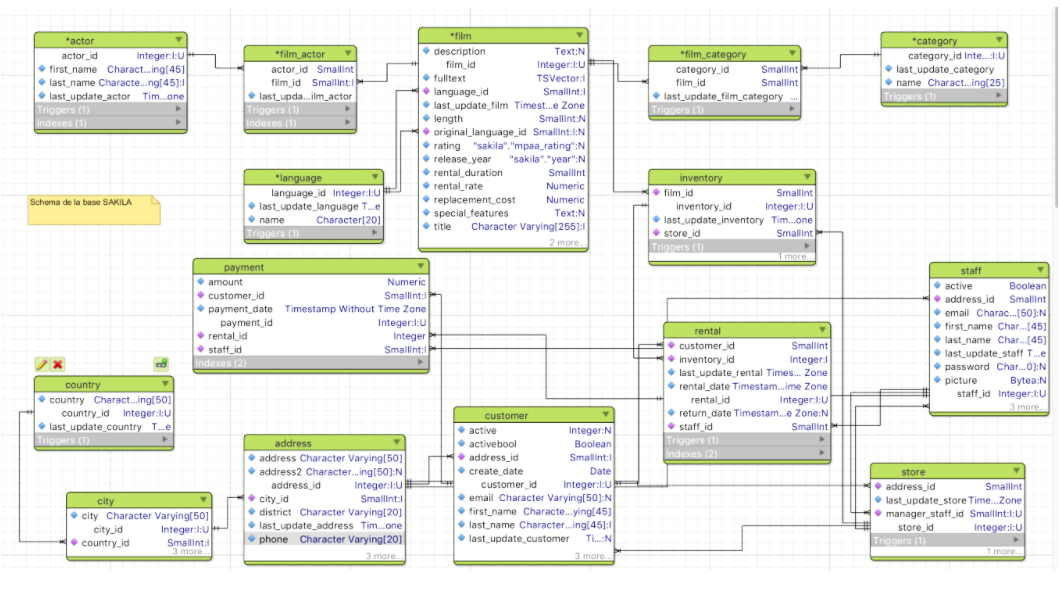
\includegraphics[scale = 0.6]{schema.PNG}
\caption{Visual example of Sakila database schema}
\end{figure}

\section*{SQL queries}
\begin{enumerate}
	\item List names of all the languages in the database (sorted alphabetically)?\\
	\begin{lstlisting}{showstringspaces=false}[language=SQL]
SELECT * FROM language
ORDER BY name ASC;
	\end{lstlisting}
	
	\item List full names of actors with "GER" in their last name, ordered by their first name.\\
	\begin{lstlisting}{showstringspaces=false}
SELECT CONCAT(first_name," ",last_name) AS full_name
FROM actor
WHERE last_name LIKE "%GER%"
ORDER BY first_name ASC;
	\end{lstlisting}
	
	\item Find all the addresses where postal code starts with "57", and return addresses sorted.
	\begin{lstlisting}{showstringspaces=false}
SELECT *
FROM address
WHERE postal_code LIKE "57%"
ORDER BY address;
	\end{lstlisting}
	
	\item How many films involve a "DWARF" in their titles?
	
	\begin{lstlisting}{showstringspaces=false}
SELECT COUNT(*) 
FROM film
WHERE title LIKE "%DWARF%";
	\end{lstlisting}
	
	\item Find full names of actors who played in a film involving 'WAR' in title and longer than 2.5 hours, along with the title, run length and release year of the movie, sorted by the actors' last names. 
	
	\begin{lstlisting}{showstringspaces=false}
SELECT CONCAT(first_name, " ",  last_name ) AS full_name,
title, release_year, length
FROM actor 
JOIN film_actor ON actor.actor_id=film_actor.actor_id
JOIN film ON film.film_id = film_actor.film_id
WHERE title LIKE '%WAR%' AND length > 150
ORDER BY last_name;
	\end{lstlisting}

	\item Find all the film categories in which there are between 55 and 65 films. Return the names of these categories and the number of films per category, sorted by the number of films descending.
	
	\begin{lstlisting}{showstringspaces=false}
CREATE VIEW R6 AS
SELECT film_category.category_id, category.name, 
COUNT(film_category.category_id) as countfilm	
FROM film_category
JOIN category 
ON film_category.category_id = category.category_id 
GROUP BY category_id;
		   
SELECT name, countfilm 
FROM R6 
WHERE countfilm > 55 AND countfilm < 65
ORDER BY countfilm DESC;
	\end{lstlisting}

	\item In how many film categories is the average difference between the film replacement cost and the rental rate larger than 17?
	
	\begin{lstlisting}{showstringspaces=false}
SELECT COUNT(*)
FROM (SELECT category_id  
FROM film 
JOIN film_category 
ON film.film_id = film_category.film_id
GROUP BY film_category.category_id
HAVING ABS(AVG(replacement_cost)) - AVG(rental_rate)>17 ) AS R7;
	\end{lstlisting}

	\item Find the address district(s) name(s) such that the minimal postal code in the district(s) is maximal over all the districts. Make sure your query ignores empty postal codes and district names.
	
	\begin{lstlisting}{showstringspaces=false}
SELECT R7.district, MAX(postcode)
FROM (SELECT district, MIN(postal_code) AS postcode 
FROM address 
WHERE postal_code IS NOT NULL AND district IS NOT NULL
GROUP BY district 
ORDER BY MIN(postal_code) DESC) AS R7;
   
	\end{lstlisting}
		
	\item Find the names (first and last) of all the actors and customers whose first name is the same as the first name of the actor with ID 101 (exclude the actor with ID 101).
	
	\begin{lstlisting}{showstringspaces=false}
SELECT first_name, last_name
FROM customer 
WHERE customer.first_name = (SELECT first_name
FROM actor WHERE actor_id = 101)
UNION
SELECT first_name, last_name FROM actor 
WHERE first_name = (SELECT first_name 
FROM actor WHERE actor_id =101) 
AND actor_id <> 101 ;
	
	\end{lstlisting}
			
\end{enumerate}

\section*{Results}

The figure below presents the results after implement queries (limit from 0 to 10 for some long results):\\
\begin{figure}
\centering
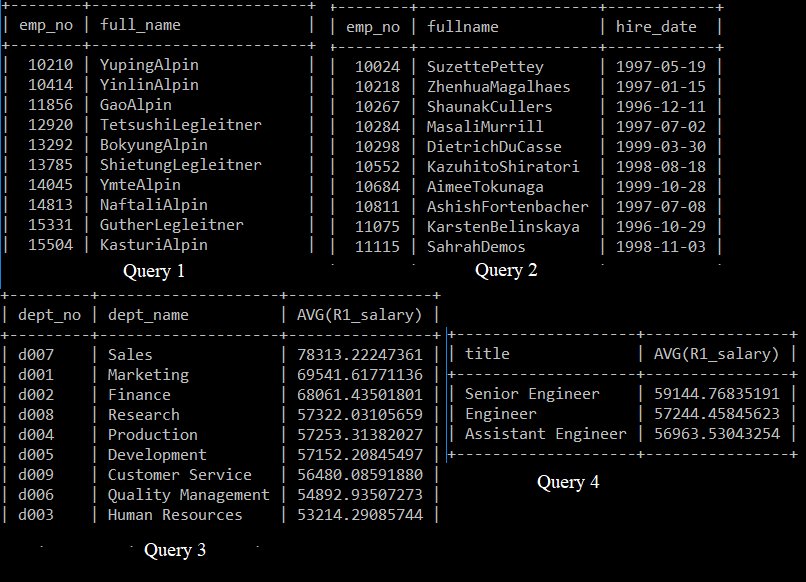
\includegraphics[scale = 0.72]{result.PNG}
\caption{Result of all queries except query 3}
\end{figure}

\begin{figure}
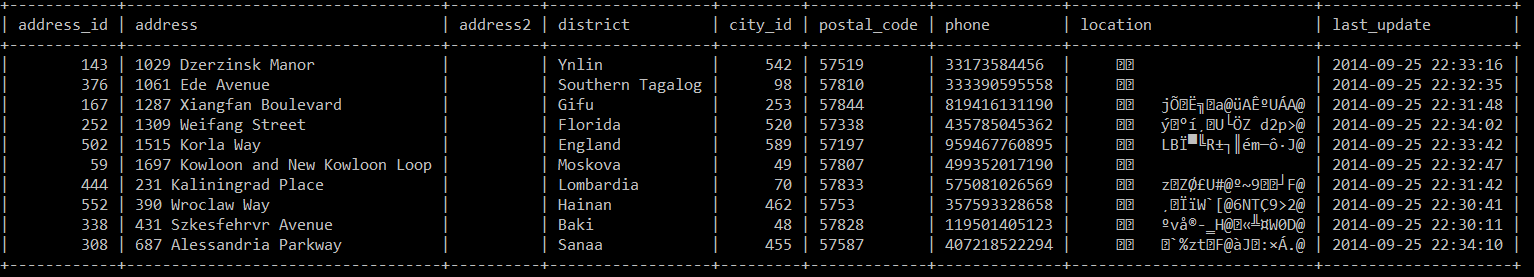
\includegraphics[scale = 0.45]{result3.PNG}
\caption{Results of query 3}
\end{figure}

\end{document}
